\chapter{Sentiment Analysis}   
	Il nostro primo obiettivo è quello di studiare l'intrattenimento, in particolare quali siano i prodotti più recensiti all'interno delle nostre quattro categorie. Come primo passo abbiamo  quindi scelto di effettuare lo studio su un numero limitato di prodotti, riducendoli a duecento, e di analizzare la loro distribuzione. I risultati ottenuti sono presentati nella Figura \ref{fig:pie_category}
	
	
	\textbf{DATASET REVIEWS????????????????????????????????????????}
		
	\begin{figure} [h]
		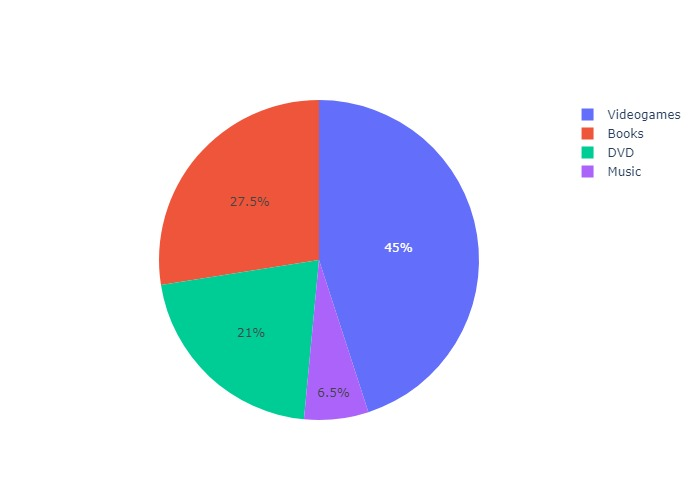
\includegraphics[width=\textwidth]{Figure/pie_category}	
		\caption{Distribuzione delle recensioni per ogni categoria.}
		\label{fig:pie_category}
	\end{figure}
	
	Dalla figura è possibile notare che, in percentuale, i prodotti più recensiti appartengono alla categoria dei videogiochi (\verb|45%|), seguiti dai libri (\verb|27.5%|), dai dvd (\verb|21%|) e dalla musica (\verb|6.5%|). Quest'ultima categoria è davvero esigua perché delle analisi diano risultati consistenti e si possano ricavare informazioni utili; inoltre poiché lo studio su cui abbiamo posto l'attenzione riguardava i più popolari, non aveva senso esaminare dei prodotti quasi privi di recensioni. Da questa considerazione è derivata la scelta di escludere \verb|music| e procedere ad analizzare l'intrattenimento solo sulle tre migliori categorie, quindi \verb|videogames|, \verb|books| e \verb|dvd|. Arrivati a questo punto il nostro studio è stato diviso in due diversi passaggi, durante i quali abbiamo cercato di rispondere a due domande ovvero quali siano i prodotti più recensiti e perché proprio loro. 
		
	\section{Primo passaggio: distribuzione del sentiment}
		Come già accennato, per poter valutare la polarità di una recensione è necessario calcolare il \textit{sentiment}. Abbiamo visto che questo calcolo può essere eseguito secondo diverse metodologie, tuttavia il nostro \textit{dataset} relativo ai prodotti, presentava al suo interno un campo che ben si prestava a questo tipo di analisi. L'attributo in questione è quello delle stelle. \textit{Amazon} infatti per ogni recensione riferita a un determinato prodotto associa una valutazione in stelle da \verb|0| a \verb|5|. Questo ha permesso di effettuare un conteggio per ogni prodotto di tutte le sue recensioni, dividendole in positive negative e neutre, secondo lo schema di seguito.
			
		\begin{itemize}
			\item \textbf{positive:} la recensione aveva un punteggio di maggiore di tre stelle.
			\item \textbf{neuter:} la recensione aveva un punteggio uguale a tre stelle.
			\item \textbf{negative:} la recensione aveva un punteggio minore di tre stelle.
		\end{itemize}
			
		Procedendo secondo queste modalità, preso per esempio il prodotto "Zelda", con \verb|200| recensioni, si calcolano quante di queste sono risultate positive negative oppure neutre e un possibile risultato potrebbe essere costituito da \verb|100| recensioni positive, \verb|70| negative e \verb|30| neutre. \\		
		Ottenuto questo elenco abbiamo calcolato la distribuzione probabilistica associata alle tre diverse polarità. In particolare per ognuna associata a uno specifico prodotto, abbiamo effettuato un rapporto tra il conteggio delle recensioni positive e negative, escludendo le neutre (dato non rilevante per la nostra analisi) e il numero di recensioni totali. 
			
		La distribuzione probabilistica della polarità ottenuta è stata quindi combinata al sottoinsieme dei prodotti più recensiti/più popolari e il risultato di questo \textit{match} è stata l'identificazione per ogni categoria dei primi cinque prodotti più popolari suddivisi in due elenchi. Il primo contenente i prodotti valutati più negativamente e nel secondo quelli valutati più positivamente. \\
		I risultati ottenuti sono visibili nelle Figure \ref{fig:top_pos_book_table} \ref{fig:top_neg_book_table}, \ref{fig:top_pos_film_table}, \ref{fig:top_neg_film_table}, \ref{fig:top_pos_videogames_table}, \ref{fig:top_neg_videogames_table}.
			
		\begin{figure} [h]
			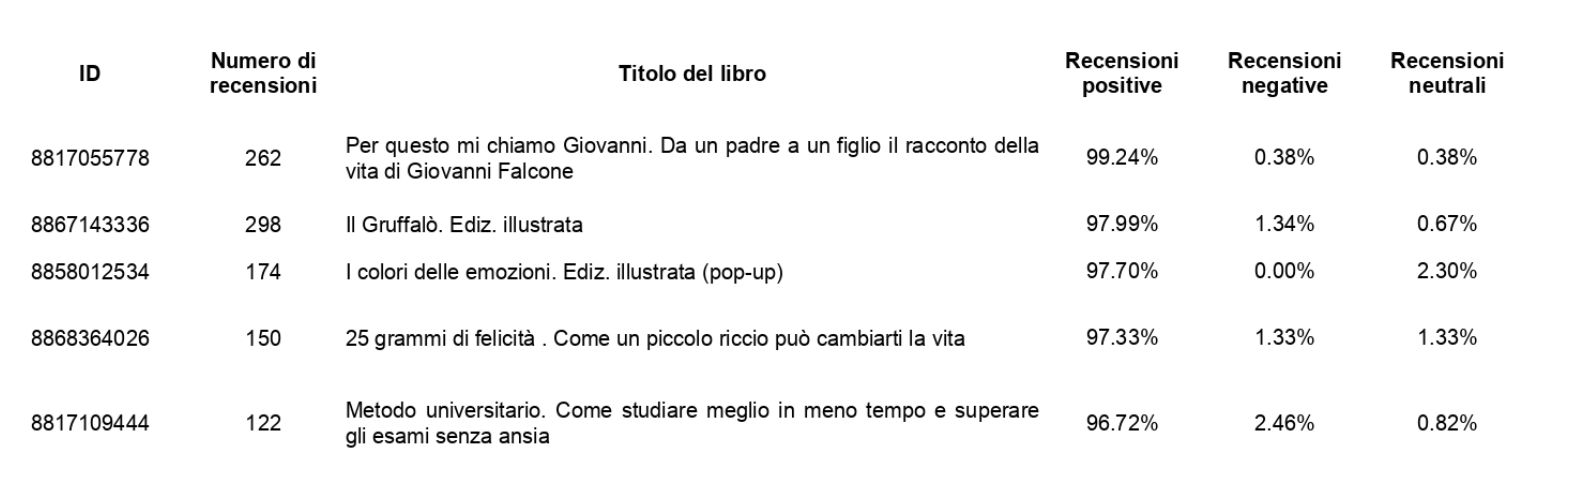
\includegraphics[width=\textwidth]{Figure/top_pos_book_table}
			\caption{Primi cinque libri con più recensioni positive}
			\label{fig:top_pos_book_table}
		\end{figure}
			
		\begin{figure} [h]
			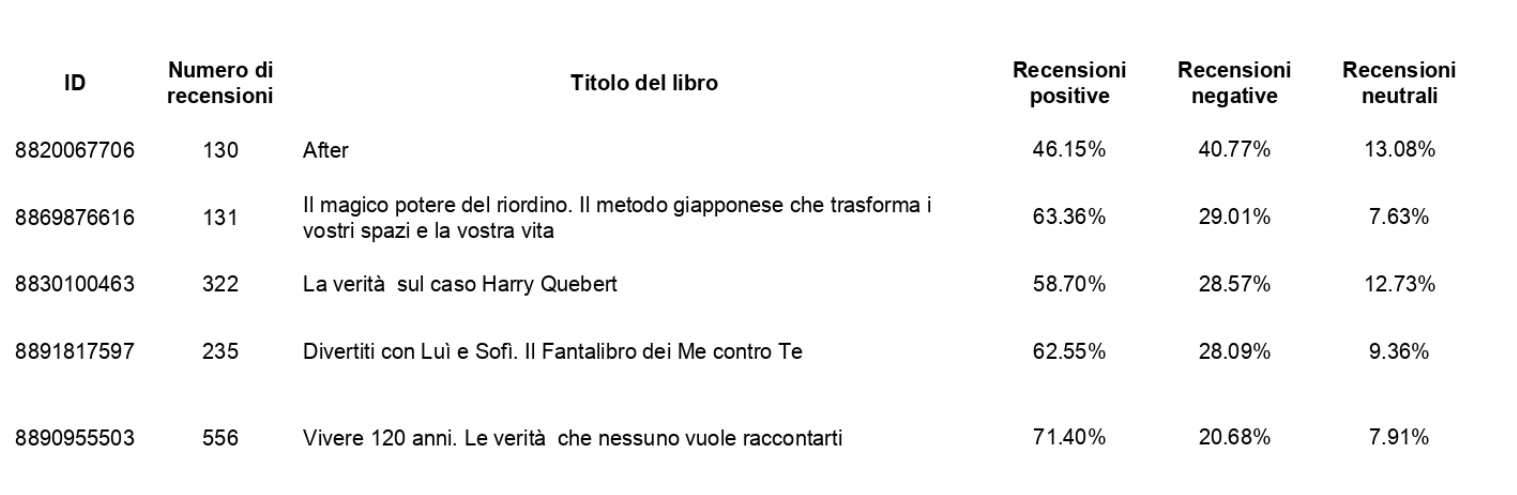
\includegraphics[width=\textwidth]{Figure/top_neg_book_table}
			\caption{Primi cinque libri con più recensioni negative}
			\label{fig:top_neg_book_table}
		\end{figure}
		
		\begin{figure} [h]
			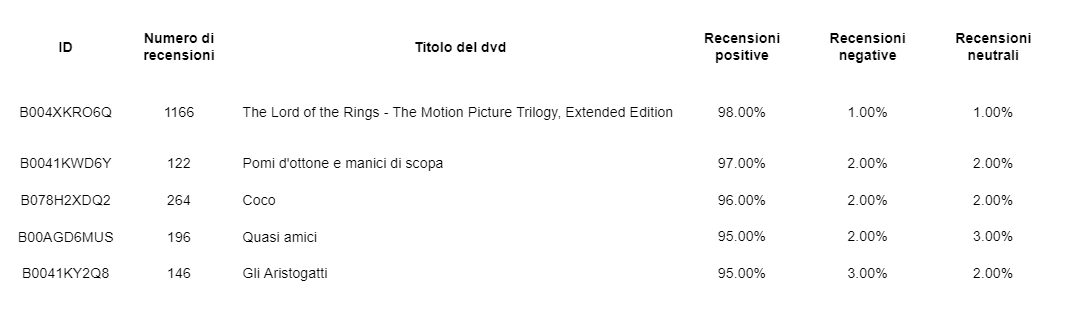
\includegraphics[width=\textwidth]{Figure/top_pos_film_table}
			\caption{Primi cinque dvd con più recensioni positive}
			\label{fig:top_pos_film_table}
		\end{figure}
		
		\begin{figure} [h]
			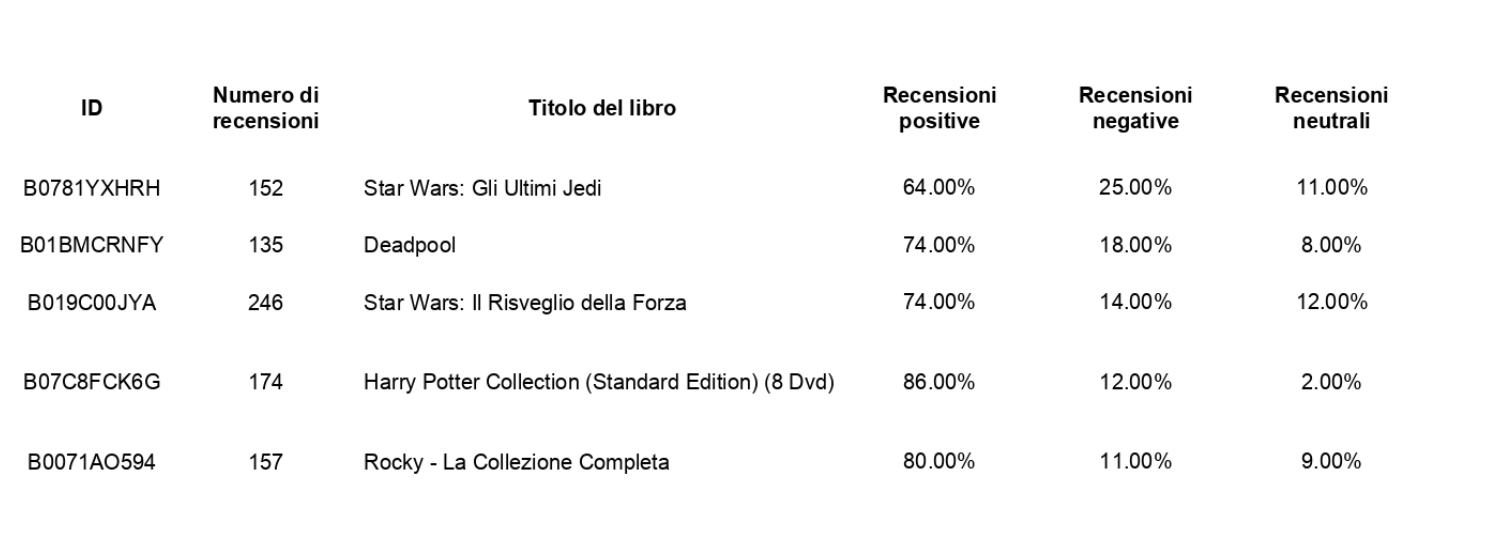
\includegraphics[width=\textwidth]{Figure/top_neg_film_table}
			\caption{Primi cinque dvd con più recensioni negative}
			\label{fig:top_neg_film_table}
		\end{figure}
		
		\begin{figure} [h]
			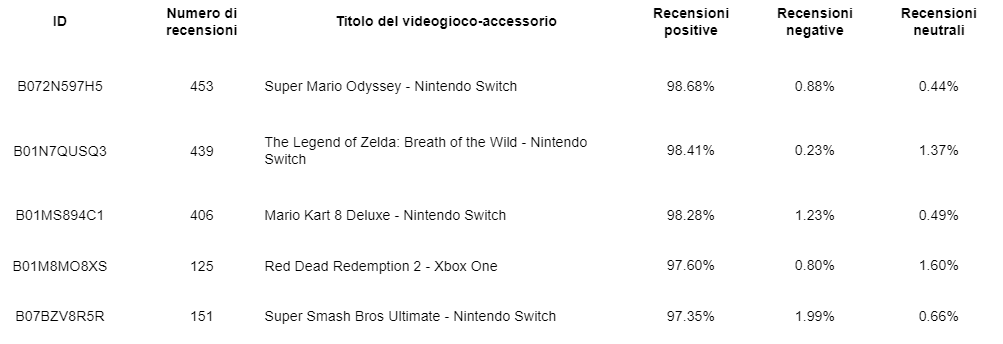
\includegraphics[width=\textwidth]{Figure/top_pos_videogames_table}
			\caption{Primi cinque videogiochi con più recensioni positive}
			\label{fig:top_pos_videogames_table}
		\end{figure}
		
		\begin{figure} [h]
			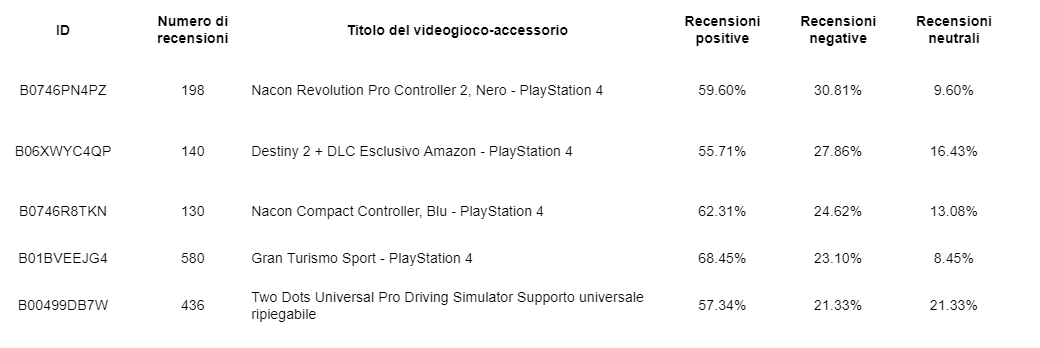
\includegraphics[width=\textwidth]{Figure/top_neg_videogames_table}
			\caption{Primi cinque videogiochi con più recensioni negative}
			\label{fig:top_neg_videogames_table}
		\end{figure}
		
	
	\section{Secondo passaggio: analisi delle parole più usate}
		Avendo risposto al primo quesito ci siamo potuti soffermare sulla seconda interrogazione, ovvero perché fossero risultati proprio questi prodotti. Siamo così andati alla ricerca delle parole più utilizzate all'interno delle recensioni (negative e positive), cercando una corrispondenza tra queste e i prodotti migliori. Tuttavia per poter eseguire questo confronto sono state necessarie delle operazioni atte a uniformare il \textit{dataset}; i dati infatti non sempre sono puliti, in essi sono presenti errori di battitura, intere frasi scritte in maiuscolo, eccessiva punteggiatura, etc. Ecco dunque il motivo del termine "uniformare", intendiamo con esso il processo di riscrittura delle frasi seguendo degli specifici passaggi, che saranno descritti nel seguito.
			
		\begin{description}
			\item[tokenizzazione:] suddivide un testo in singole parole, i\textit{token}), che saranno utilizzati per altri tipi di analisi o attività.
			\item[standardizzazione:] riscrittura delle parole da \textit{upper case} a \textit{lower case}. 
			\item[rimozione delle \textit{stopwords},] parole comuni prive di significato, ma che ricorrono spesso all'interno della frasi.
			\item[rimozione delle cifre numeriche]
			\item[rimozione della punteggiatura,] tuttavia nella nostra implementazione questa fase è subentrata all'interno della \verb|tokenizzazione|. 
			\item [stemming:] processo di riduzione delle parole flesse (o talvolta derivate) alla loro forma di origine, base o radice.
		\end{description}
			
		Al termine del processo, l'\textit{output} risultante era composto da un elenco di parole scritte Italiano corretto, privo di segni di punteggiatura o numeri, scritto in forma minuscola, ridotto alla radice. A questo punto è stato quindi possibile effettuare un'operazione di visualizzazioni delle parole più usate all'interno delle recensioni, per comprendere il motivo per cui proprio quei prodotti presenti nella lista rientrino nei migliori, per entrambe le polarità. La tecnica visiva utilizzata è quella dei \verb|wordclouds|, che consiste nella raccolta delle parole più usate nelle recensioni (\verb|word|), rappresentate per mezzo di \verb|cloud|, ha permesso di confrontare le recensioni positive e negative per ogni categoria e di comprendere che cosa determinava l'appartenenza dei prodotti all'insieme dei "migliori" o dei peggiori. 
		
		\subsection{Wordclouds libri} 
			Nella Figura \ref{fig:wordclouds_book} sono mostrati i \textit{wordclouds} ottenuti per la categoria libri. In particolare l'immagine di sinistra rappresenta le parole più usate nelle recensioni positive, mentre a destra sono rappresentate quelle negative. 
			
			\begin{figure} [h]
				\centering
				\begin{subfigure}{0.48\textwidth}
					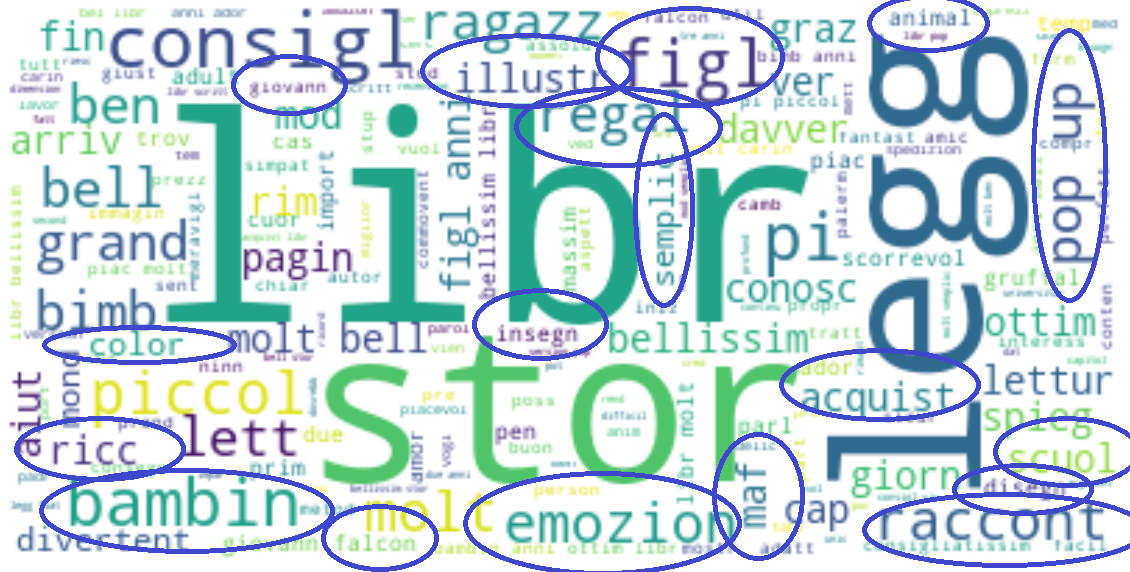
\includegraphics[width=\textwidth]{Figure/top_positive_books}
					\caption{Recensioni positive}
					\label{fig:top_positive_books}
				\end{subfigure}
				\begin{subfigure}{0.48\textwidth}
					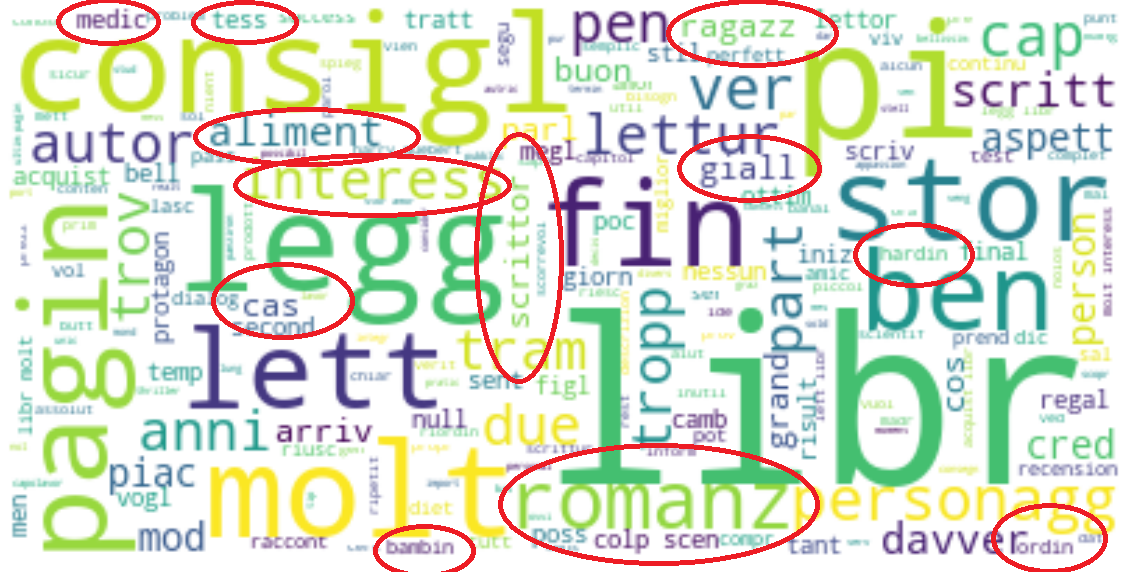
\includegraphics[width=\textwidth]{Figure/top_negative_books}
					\caption{Recensioni negative}
					\label{fig:top_negative_books}
				\end{subfigure}
				\caption{Wordclouds libri}\label{fig:wordclouds_book}
			\end{figure}
			
			\begin{description}
				\item[Recensioni positive:]
				 nello schema sono rappresentate con dimensione maggiore le parole \verb|libr|, \verb|stori|, \verb|legg|, a dimostrazione del fatto che queste sono in assoluto le parole più frequenti all'interno delle recensioni degli utenti. Non sorprende che i tre termini si riferiscano alla categoria selezionata, nel caso attuale quella dei libri; vedremo che questo comportamento ricorrerà sempre durante l'analisi tramite textit{wordclouds}. Concentriamoci invece sulle parole che racchiudono informazioni, ricordando che l'obiettivo primario è comprendere perché i libri di Figura \ref{fig:top_pos_book_table} siano risultati i migliori.
				\begin{itemize}
					\item \texttt{ricc}, \texttt{figl}, \texttt{falcon},  \texttt{giovann}, \texttt{"emozion"}, \texttt{pop up}: \\
					sono tutte parole presenti in alcuni dei titoli della lista dei migliori, in ordine \textit{"Per questo mi chiamo Giovanni. da un padre a un figlio il racconto della vita di Giovanni Falcone"}, \textit{"I colori delle emozioni (pop-up)"}, "\textit{25 grammi di felicità - Come un piccolo riccio può cambiarti la vita}". 
					\item \texttt{maf}: \\
					termine che se esteso indica la mafia, riferito quindi al primo libro dell'elenco.
					\item \texttt{illustr}, \texttt{bambin}, \texttt{color}, \texttt{semplic},  \texttt{disegn}, \texttt{raccont}, \texttt{animal} : \\
					sono tutti termini riguardanti l'infanzia. Da questa informazioni comprendiamo che la maggior parte delle recensioni commenta positivamente i libri per bambini, che sono semplici, colorati, ricchi di disegni e di racconti basati sugli animali. Quindi questi vocaboli sono riferiti per lo più al secondo e al terzo libro dell'elenco dei migliori; tuttavia l'ultimo termine può essere esteso anche quarto prodotto. 
					\item \texttt{insegn}, \texttt{scuol}: \\
					sono vocaboli riferiti all'ambiente scolastico; quindi probabilmente riferito all'ultimo libro, criticato positivamente poiché insegna tematiche relative alla scuola.
					\item \texttt{acquist}, \texttt{regal}: \\
					molto probabilmente alcuni libri, acquistati per un regalo, hanno suscitato delle impressioni positive nell'utente, che ha quindi recensito positivamente.
				\end{itemize}	
			
				\item[Recensioni negative:] 
				nello schema sono rappresentate con dimensione maggiore le parole \verb|libr|, \verb|pagin|, \verb|legg|, a dimostrazione del fatto che queste sono in assoluto le parole più frequenti all'interno delle recensioni degli utenti. Notiamo che due su tre sono parole già trovate all'interno dell'elenco delle parole positive, poiché anche in questo caso sono termini utili a determinare la categoria in questione. Studiamo ora le altre parole in relazione all'elenco già stilato (Figura \ref{fig:top_neg_book_table}).
				
				\begin{itemize}
					\item \texttt{hardin}, \texttt{tess}, \texttt{romanz}: \\
					sono i termini più espliciti dell'insieme, indicano infatti i nomi dei protagonisti del romanzo "\textit{After}"
					\item \texttt{ordin}, \texttt{cas}:\\
					sono parole usate nel secondo prodotto dell'elenco 
					\item \texttt{scrittor}, \texttt{giall}:\\
					si riferiscono probabilmente a "\textit{La verità del caso di Harry Quebert}", un giallo che vede protagonista uno scrittore.
					\texttt{bambin}: \\
					fra tutti i prodotti dell'elenco quello che certamente si adatta alle linee giovanili è sicuramente il quarto libro dell'elenco, pieno di attività creative e non proposte ai più piccini.
					\texttt{aliment}: \\
					vocabolo riferito a "\textit{Vivere 120 anni. la verità che nessuno vuole raccontarti}".
					\texttt{medic}, \texttt{ragazz}, \texttt{interessant}: \\
					tra i proposti sono quelli che più di tutti racchiudono le possibili cause di una critica. Il libro, presupponibilmente l'ultimo dell'elenco, probabilmente aveva un approccio troppo rivolto alla medicina o forse troppo poco. Il secondo è forse più rivolto ad "\textit{After}", criticato spesso per rivolgersi esclusivamente a un pubblico femminile. Più generico, invece, è il vocabolo \verb|interessante|, che ben si adatta a ognuno dei prodotti proposti.												
				\end{itemize}
			\end{description}
		
		
		\subsection{Wordclouds dvd}
			Nella Figura \ref{fig:wordclouds_dvd} sono mostrati i \textit{wordclouds} ottenuti per la categoria dvd. In particolare l'immagine di sinistra rappresenta le parole più usate nelle recensioni positive, mentre a destra sono rappresentate quelle negative. 
				
			\begin{figure} [h]
				\centering
				\begin{subfigure}{0.48\textwidth}
					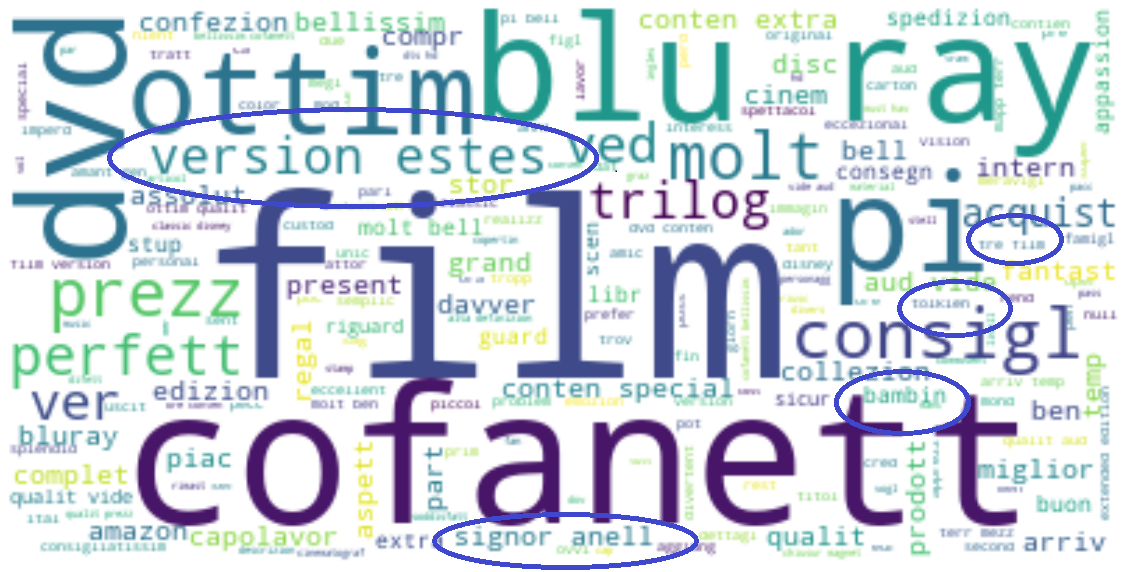
\includegraphics[width=\textwidth]{Figure/top_positive_dvd}
					\caption{Recensioni positive}
					\label{fig:top_positive_dvd}
				\end{subfigure}
				\begin{subfigure}{0.48\textwidth}
					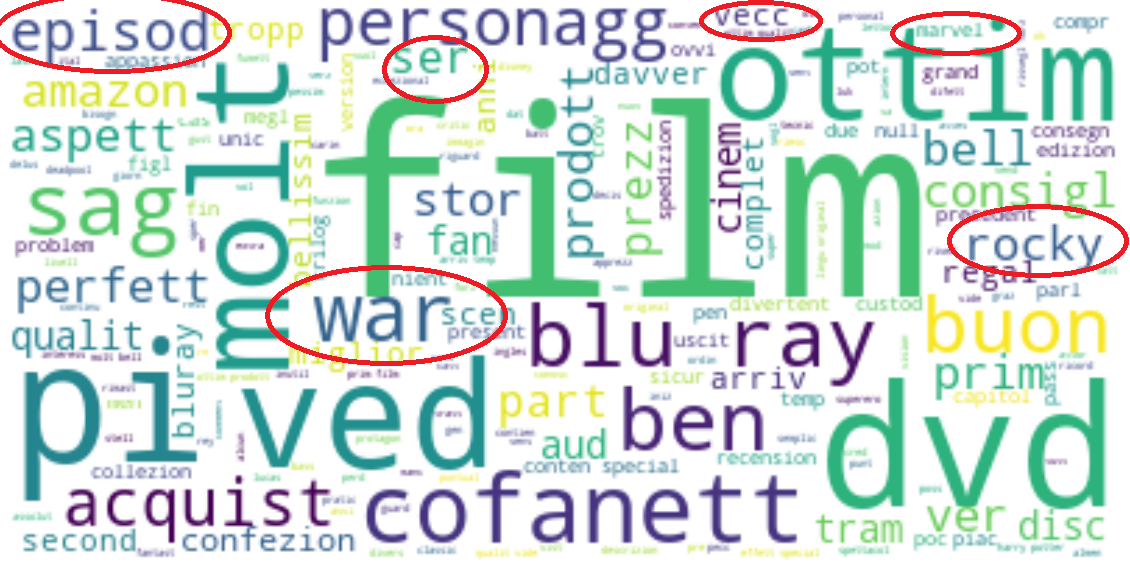
\includegraphics[width=\textwidth]{Figure/top_negative_dvd}
					\caption{Recensioni negative}
					\label{fig:top_negative_dvd}
				\end{subfigure}
				\caption{Wordclouds dvd}\label{fig:wordclouds_dvd}
			\end{figure}
		
			\begin{description}
				\item[Recensioni positive:]
				nello schema sono rappresentate con dimensione maggiore le parole \verb|dvd|, \verb|film|, \verb|blu ray|, riferite genericamente alla categoria presa in esame. 	
				\begin{itemize}
					\item \texttt{signore anell}, \texttt{tolkien}, \texttt{tre film}: \\
					I termini selezionati sono accomunati dalla tematica "\textit{Signore degli Anelli}", trilogia ispirato all'omonimo romanzo scritto da \textit{Tolkien}, che ha raccolto molti consensi, dato che più parole lo caratterizzano.
					\item \texttt{bambin}: \\
					I dvd criticati positivamente sono stati quelli adatti a un giovane pubblico. Da notare che il termine risponde ancora alle caratteristiche del "\textit{Signore degli Anelli}".
					\item \texttt{version estes}: \\
					Tra i tanti comprati o visti, i dvd in versione estesa hanno riscontrato un consenso positivo.
				\end{itemize}	
				
				Si noti che le parole trovate ben si accordano con i risultati trovati nei passaggi precedenti (Figura \ref{fig:top_pos_film_table}), dove il miglior prodotto era la trilogia del \textit{"Signore degli anelli}", seguito poi da altri film adatti ai bambini ("\textit{Coco}", terzo posto, e "\textit{Gli Aristogatti}", ultimo posto, sono addirittura dei cartoni animati).
					
				\item[Recensioni negative:] 
				nello schema i termini generici riscontrabili con la categoria in questione sono \verb|film|, \verb|dvd |, \verb|blu ray|. Poiché nella Figura \ref{fig:top_neg_film_table}, abbiamo trovato cinque prodotti di diversa natura come maggiormente criticati, ci aspettiamo di trovare termini che li identifichino e che argomentino le recensioni negative.
				\begin{itemize}
					\item \texttt{war}, \texttt{marvel}, \texttt{rocky}: \\
					sono tutti termini utili a identificare il dvd in questione. Come ci aspettavamo, il primo di questi si riferisce al film di "\textit{Star Wars}", il primo peggio criticato, il secondo invece riguarda "\textit{Deadpool}", un film della marvel e il terzo del film "\textit{Rocky}". 
					\item \texttt{ser}, \texttt{episod}, \texttt{vecc}: \\
					In queste parole sono racchiuse le cause delle critiche. I primi due probabilmente rivolti a "\textit{Star Wars}", una serie di nove film, ognuno dei quali denominato con il termine di "episodio". Il terzo vocabolo, che molto probabilmente si rifesce a "\textit{Rocky}", criticato invece per l'età.		
				\end{itemize}
			\end{description}
		
		
		\subsection{Wordclouds videogiochi}
			Nella Figura \ref{fig:wordclouds_videogames} sono mostrati i \textit{wordclouds} ottenuti per la categoria videogiochi. In particolare l'immagine di sinistra rappresenta le parole più usate nelle recensioni positive, mentre a destra sono rappresentate quelle negative. 
			
			\begin{figure} [h]
				\centering
				\begin{subfigure}{0.48\textwidth}
					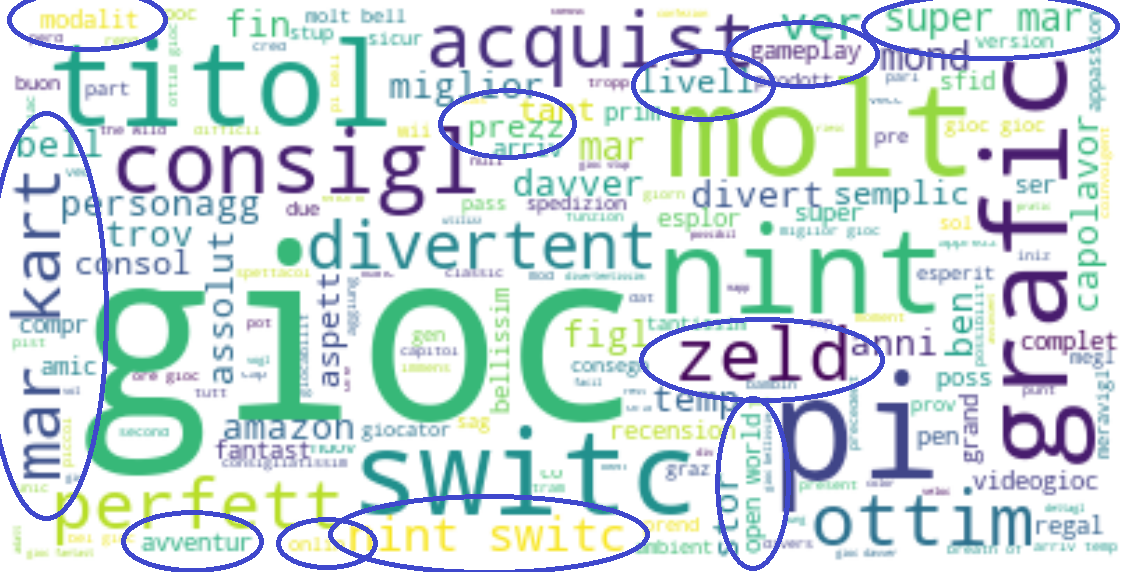
\includegraphics[width=\textwidth]{Figure/top_positive_videogames}
					\caption{Recensioni positive}
					\label{fig:top_positive_videogames}
				\end{subfigure}
				\begin{subfigure}{0.48\textwidth}
					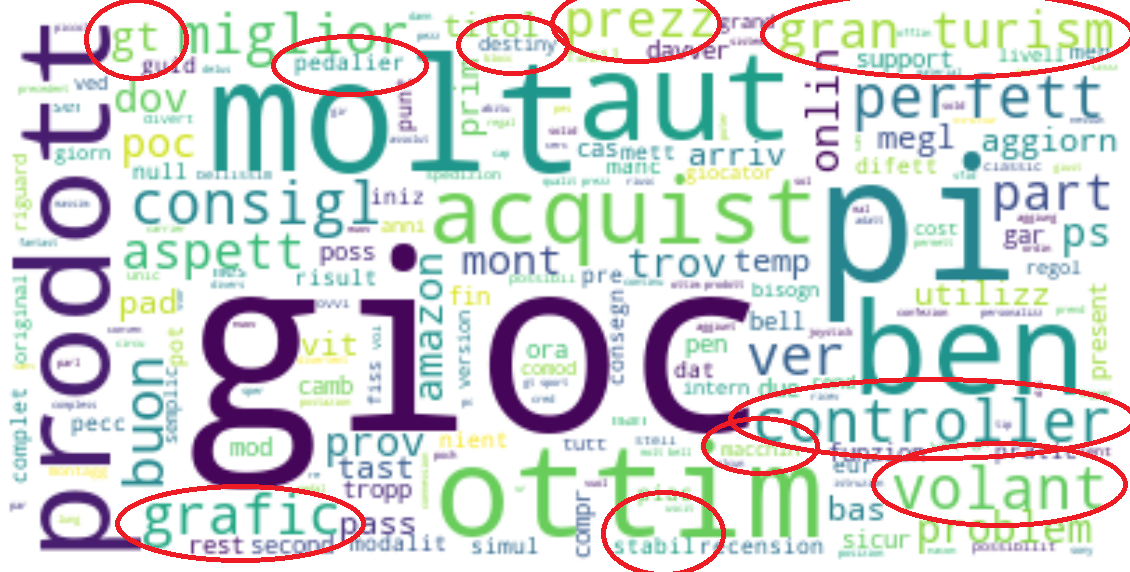
\includegraphics[width=\textwidth]{Figure/top_negative_videogames}
					\caption{Recensioni negative}
					\label{fig:top_negative_videogames}
				\end{subfigure}
				\caption{Wordclouds videogiochi}\label{fig:wordclouds_videogames}
			\end{figure}
			
			\begin{description}
				\item[Recensioni positive:]
				nello schema sono rappresentate con dimensione maggiore le parole \verb|gioc|, \verb|grafic|, riferite genericamente alla categoria presa in esame, di cui si apprezza la natura del gioco e la grafica. Per quanto riguarda invece il contenuto informativo, soffermiamoci sulla Figura \ref{fig:top_pos_videogames_table}; dalla quale apprendiamo quali sono i cinque prodotti migliori e cerchiamo di ricostruire cosa li caratterizza.
				\begin{itemize}
					\item \texttt{super mar}, \texttt{mar kart}, \texttt{zeld}: \\
					I termini selezionati rappresentano infatti il podio dei migliori, rispettivamente "\textit{Super Mario Odyssey}", "\textit{The Legend of Zelda}" e \textit{Mario Kart 8 Deluxe}". 
					\item \texttt{nint switch}: \\
					i videogiochi più apprezzati sono quelli per \textit{ninntendo switch}; non a caso infatti i tre migliori sono proprio accomunati da questa caratteristica.
					\item \texttt{avventur}, \texttt{online}, \texttt{modalit}, \texttt{open world}, \texttt{livell}, \texttt{gameplay}: \\
					tutti questi vocaboli sono caratteristiche positive dei giochi; probabilmente apprezzati quindi dalle avventure proposte dalla storia, dalla possibilità di giocare online in più modalità, compresa anche quella esplorativa, organizzate in livelli o dal \textit{gameplay} intuitivo, etc.
					\item \texttt{prezz}: l'appartenenza dei giochi alla lista dei migliori può anche essere stata determinata dal prezzo, trovato forse dagli utenti accessibile o anche basso.
				\end{itemize}	
								
				\item[Recensioni negative:] 
				nello schema i termini generici più rilevanti per la categoria sono \verb|gioc|, \verb|prodott|. Concentriamoci ora sulla \textit{top five} dei prodotti negativi (Figura \ref{fig:top_neg_videogames_table}), contrariamente ai casi precedenti abbiamo rappresentati tra i pprimi cinque prodotti ci sono sia videogiochi, sia accessori appartenenti alla categoria in questione.
				\begin{itemize}
					\item \texttt{gran turism}, \texttt{destiny}, \texttt{controller}: \\
					sono tutti termini appartenenti all'elenco dei primi cinque prodotti con più recensioni negative. 
					\item \texttt{gt}, \texttt{pedalier}, \texttt{macchin}, \texttt{volant}: \\
					Sono parole riferite al gioco di corse automobilistiche "\textit{Grand Turism}", apprezzato soprattutto quando si gioca con un volante o una pedaliera. 
					\item \texttt{grafic}, \texttt{stabil}: 
					i giochi sono probabilmente apprezzati per la grafica efficace e con il termine \verb|stabile| ci si vuole forse riferire alla qualità da parte del gioco di  mantenere la fluidità dell'immagine priva di scatti, o anche la capacità del gioco di non "\textit{crashare}".
					\item \texttt{prezz}: 
					anche in questo caso il prodotto è stato recensito rispetto al suo prezzo, contrariamente a prima però questa volta trovato troppo alto.
				\end{itemize}
			\end{description}
			
	\section{Correlazione tra prezzo e sentiment}
		Avendo trovato un riscontro positivo alle domande poste, siamo passati a una seconda analisi del \textit{sentiment} sul \textit{dataset} prodotti. In particolare ci siamo chiesti se il prezzo associato a ogni prodotto, fosse determinante per la polarità delle recensioni. Esiste infatti un'idea duale legato a un prezzo ridotto o eccessivo. Nel primo caso un prezzo ridotto può essere fonte di:
		
		\begin{itemize}
			\item \textbf{reazioni positive}, legate all'esigua quantità di denaro spesa per un prodotto funzionante.
			\item \textbf{reazioni negative}, legate alla qualità infima dei materiali.
		\end{itemize}
	
		Medesimo comportamento è legato ad alti costi. In questo caso abbiamo:
		
		\begin{itemize}
			\item \textbf{reazioni positive}, perché il prodotto oltre che essere funzionante è di ottima qualità.
			\item \textbf{reazioni negative}, dovute al costo eccessivo di alcuni prodotti, dove si paga non tanto la qualità, quanto piuttosto il marchio.
		\end{itemize}
	
		Contrariamente a quanto è stato compiuto per le prime analisi, ora non si è eseguita una campionatura sui prodotti migliori, ma è stato calcolato il sentiment, secondo le modalità precedente descritte, per ogni prodotto. Questo sentiment è stato poi raccolto in base alle categorie, sviluppando ancora una volta due gruppi di insiemi, per le recensioni positive e negative, questa volta però sull'intero \textit{set} di prodotti. Ad operazione conclusa abbiamo raccolto tutti i possibili prezzi per ogni categoria e li abbiamo suddivisi in intervalli, così che per esempio, per la categoria libri ci fosse, tra i tanti, l'intervallo \verb|[1-10]| che racchiudesse al suo interno tutti i prodotti con un prezzo compreso tra il valore \verb|0| e il valore \verb|10|. 

		Una volta ottenuti i sotto-raggruppamenti dei prezzi per ogni categoria, siamo andati a visualizzare la tipologia delle recensioni per ognuno di essi. In particolare, tramite un istogramma, abbiamo rappresentato sull'asse delle ascisse tutti gli intervalli per una certa categoria e sull'asse delle ordinate la valutazione totale sulle recensioni in percentuale. Analizziamo i risultati per ogni categoria.
		
		\subsection{Categoria libri}
			Per la categoria "libri", abbiamo il \verb|???| composto da recensioni positive, mentre le restanti sono negative, come mostrato in Figura ??????
			Studiamo come queste sono distribuite in base al prezzo, più precisamente all'intervallo di prezzi. \\
			Dalla Figura \ref{fig:priceVSrating_books} si evince che le recensioni positive sono maggiormente distribuite nei prodotti con un prezzo che oscilla tra \verb|0| e \verb|15| euro. Andando avanti la percentuale diminuisce, fino a non avere esemplari su un range dal valore compreso tra i \verb|100| e \verb|150| euro. Per quanto riguarda le recensioni negative, invece, si riscontra una presenza dominante tra quelle appartenenti al primo intervallo, cala drasticamente nel secondo fino a non avere prodotti per i tre \textit{range} successivi. Una possibile chiave di lettura per questa rappresentazione potrebbe essere che, per quanto riguarda i commenti positivi, questi siano presenti in ogni categoria perché con un prezzo basso, se l'utente è soddisfatto a maggior ragione lascerà una recensione positiva, in quanto non ha dovuto spendere molto per un prodotto funzionante. A prezzi elevati invece, è difficile che il prodotto non soddisfi le aspettative, in quanto un libro richiede pochi requisiti di qualità, ne consegue che chi spende rimane soddisfatto, pertanto i commenti negativi si concentrino solo nel primo intervallo.
		
				
			\begin{figure} [h]
				\centering
				\begin{subfigure}{0.48\textwidth}
					\includegraphics[width=\textwidth]{Figure/???}
					\caption{????}
					\label{fig:???}
				\end{subfigure}
				\begin{subfigure}{0.48\textwidth}
					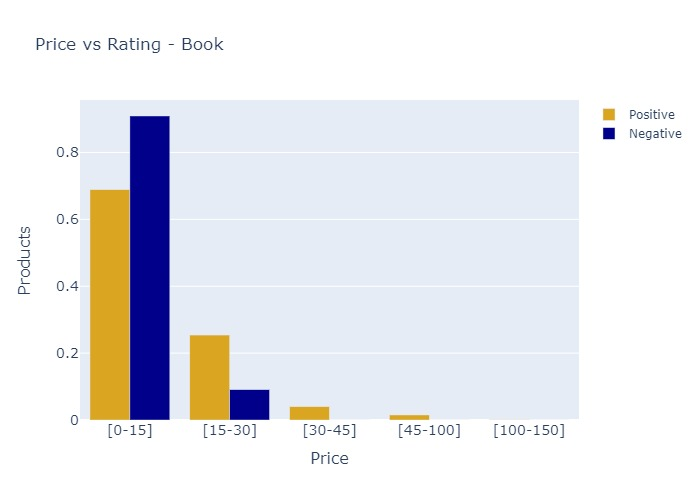
\includegraphics[width=\textwidth]{Figure/priceVSrating_books}
					\caption{Price vs raiting}
					\label{fig:priceVSrating_books}
				\end{subfigure}
				\caption{Correlazione tra prezzo e sentiment}\label{fig:price_raiting_book}
			\end{figure}
		
		
		\subsection{Categoria dvd}
		Per la categoria "dvd", abbiamo una distribuzione probabilistica di recensioni medie pari a \verb|???| per quelle positive e \verb|???| per quelle negative.
		Dalla Figura \ref{fig:priceVSrating_dvd} si può notare che il \verb|60%| delle recensioni positive appartengono al primo intervallo, diminuiscono per il secondo e terzo \textit{range}, mentre per il quarto si ha un impercettibile aumento delle stesse, probabilmente dovute al fattore qualità-prezzo. Come prima per l'ultimo intervallo abbiamo esclusivamente recensioni positive, seppur molto basse; in quanto difficilmente un utente spende grandi somme di denaro per comprare dvd. Dall'altra parte abbiamo invece quelle negative, il cui numero diminuisce all'aumentare del prezzo, ma che comunque si mantiene pressoché uguale per ogni intervallo.
		 utilizzata per i libri
		
		\begin{figure} [h]
			\centering
			\begin{subfigure}{0.48\textwidth}
				\includegraphics[width=\textwidth]{Figure/???}
				\caption{????}
				\label{fig:???}
			\end{subfigure}
			\begin{subfigure}{0.48\textwidth}
				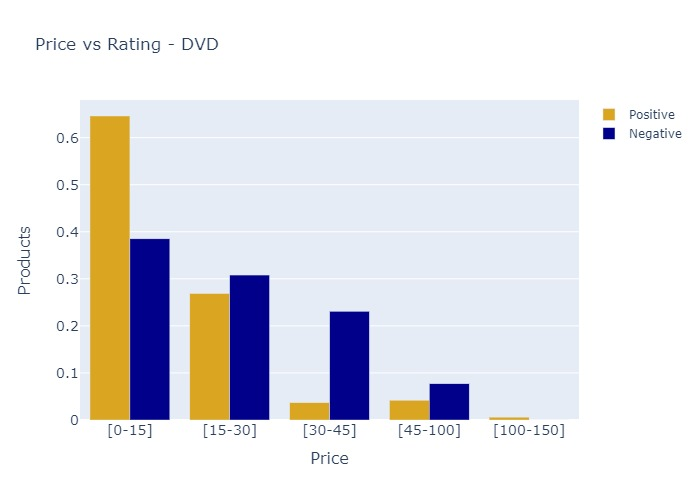
\includegraphics[width=\textwidth]{Figure/priceVSrating_dvd}
				\caption{Price vs raiting}
				\label{fig:priceVSrating_dvd}
			\end{subfigure}
			\caption{Correlazione tra prezzo e sentiment}\label{fig:price_raiting_dvd}
		\end{figure}
	
	
		\subsection{Categoria videogiochi}
			Per la categoria "videogiochi", abbiamo una distribuzione probabilistica formata da recensioni positive per il \verb|???|, mentre dal \verb|????| per quelle negative. Studiamo come queste sono distribuite in base al prezzo, più precisamente all'intervallo di prezzi\\
			Dalla Figura \ref{fig:priceVSrating_videogames} si può notare come anche in questo caso il comportamento per le recensioni positive sia a discesa, con più del \verb|50%| concentrate nel primo intervallo. Per quelle negative invece abbiamo una percentuale più o meno simile per i primi due intervalli, cala proseguendo, fino a scomparire del tutto nell'ultimo intervallo. Anche in questo caso la chiave di lettura può essere la stessa utilizzata per i libri.
		
		
		Dalla Figura \ref{fig:priceVSrating_videogames} si evince che ...
		
		\begin{figure} [h]
			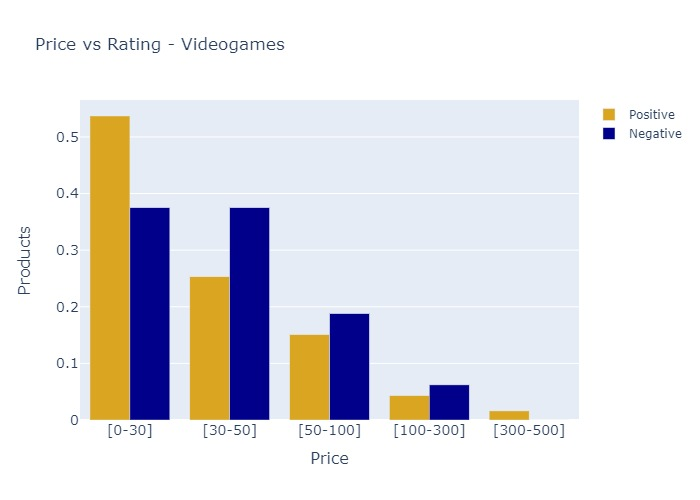
\includegraphics[width=\textwidth]{Figure/priceVSrating_videogames}
			\caption{Istogramma relazione prezzo e valutazione recensioni.}
			\label{fig:priceVSrating_videogames}
		\end{figure}
	
		
		\subsection{Categoria musica}
			Un dato importante è rappresentato dalla categoria "musica", che conta solo recensioni positive. A riprova di questo, vi è anche l'istogramma in Figura \ref{fig:???}, dove non compare il colore blu delle recensioni negative. 
				
			\begin{figure} [h]
				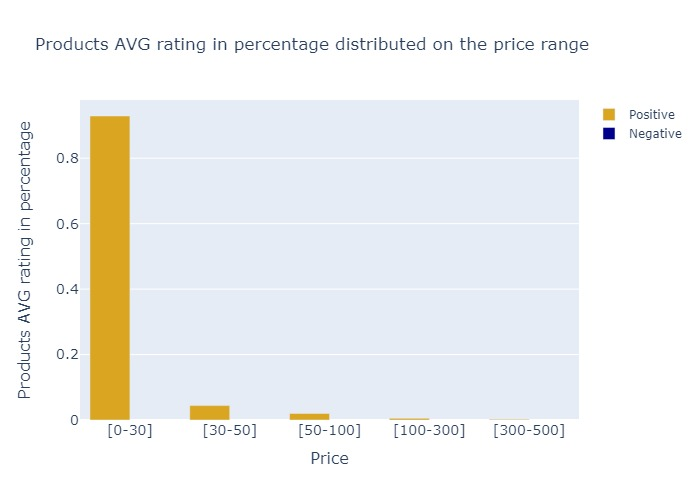
\includegraphics[width=\textwidth]{Figure/priceVSrating_music}
				\caption{Istogramma relazione prezzo e valutazione recensioni.}
				\label{fig:priceVSrating_music}
			\end{figure}
		
		
		